\chapter{Related Work} 
\label{Chapter3} 
\lhead{Chapter 3. \emph{Related Work}} 

\section{Native Client Acceleration Modules (NaClAM)} % (fold)
\label{sec:naclam}

In October 2012, John McCutchan at Google came up with the idea of using Native Client as a way to get native performance inside a normal JavaScript web application. He called it ``Native Client Acceleration Modules (NaClAM)'', with a slogan ``\emph{90\% Web App. Native Performance Where You Need It}''.

NaClAM is essentially a simple event-based RPC framework that allowed sending and receiving JavaScript objects as well as binary data. The RPC framework worked by using \emph{event listeners} and \emph{handlers} on both the JavaScript hand C++ ends. 

On the JavaScript side, a library called NaClAM.js was provided, which allowed developers to attach listeners to a particular module using the \lstinline{addEventListener(type,handler)} method. To send requests to the C++, the \lstinline{dispatchEvent} method is used. On the C++ side, messages are handled inside one overridden method called \lstinline{NaClAMModuleHandleMessage}. Here, checks are performed on the message received, and the appropriate method is called. Listing \ref{code_naclam_handle_message} shows an example of this. 

\lstset{language=C++,caption={NaClAM C++ message handler},label=code_naclam_handle_message}
\begin{code}
void NaClAMModuleHandleMessage(const NaClAMMessage& message) {
  if (message.cmdString.compare("floatsum") == 0) {
    handleFloatSum(message);
  } else if (message.cmdString.compare("addfloatarrays") == 0) {
    handleAddFloats(message);
  } else {
    NaClAMPrintf("Got message I don't understand");
  }
}
\end{code}

\subsection{Message Format} % (fold)
\label{sub:naclam_message_format}
\begin{figure}
	\centering
	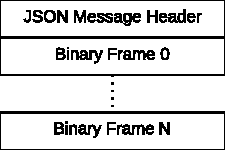
\includegraphics[width=0.3\textwidth]{naclam-msg-format.pdf} 
	\caption{A NaClAM message including binary frames}
	\label{fig:naclam_msg_format}
\end{figure}

At the message passing level, NaClAM uses JavaScript/C++ strings to transport messages. These messages hold information about the message such as the command string (like ``\lstinline{floatsum}'' in listing \ref{code_naclam_handle_message}). The strings are constructed using the jsoncpp library. 

Crucially, however, they also tell the framework how many binary \emph{frames} are expected to come after this message. Figure \ref{fig:naclam_msg_format} shows an example of a message containing $N$ frames. A frame is essentially a binary block of data sent by a separate call to \lstinline{PostMessage}. The receiver collects all the frames before triggering the event handler.

% subsection naclam_message_format (end)

\subsection{Advantages and Disadvantages} % (fold)
\label{sub:naclam_advantages_and_disadvantages}
NaClAM modules have the benefit of being simple and fast. There is a good distinction between the message information stored in the header and the message data stored as binary inside the frames. This allows developers to use the message header to implement event logic, while using the frames to transfer actual data. It also means that because the data is binary and almost no marshalling happens, the transfer speed is very fast, since binary data is \emph{shared} between JavaScript and C++.

However, there are a few issues with using NaClAM modules. The first is a lack of overall, high-level structure. The developer has to be aware and understand exactly what the framework is doing behind the scenes to write their application, which adds more burden on the developer, especially since almost no documentation is provided. The second issue is how the message header types are implemented. Although the framework allows sending application data in binary frames, the header information is sent as JSON, and is manipulated by the jsoncpp library - so another library the developer needs to get used to. Importantly, this means the developer needs to unpack and pack the data they are sending in the header section by themselves by using the jsoncpp library. Another issue is how the framework does not use a callback approach to asynchronous remote procedure calls. In other words, to `return' a value from a C++ function back to JavaScript, a \emph{different} event needs to be triggered from the C++, and handled by the JavaScript library. In other words, two different events need to be managed in both C++ and JavaScript for only one RPC call which returns data. If there are many functions like this, the developer needs to manage several different events, which is tedious. Finally, although the framework has been demoed and gained a lot of popularity, it still seems to not be well tested, as no unit tests exist for either the C++ or JavaScript implementations have been written. This makes it feel like an experimental project, rather than a full, well supported framework. 

Despite these issues, the Native Calls project was heavily influenced and inspired by the overall idea of the NaClAM project, especially its use cases and scenarios.
% subsection naclam_advantages_and_disadvantages (end)

% section naclam (end)

\section{Node.js C++ Addons} % (fold)
\label{sec:node_js_c_bindings}
Node.js is a JavaScript platform built on top of Chrome's V8 JavaScript engine that allows running JavaScript on server-side applications. Listing \ref{code_nodejs_http_server} shows an example of a node.js HTTP server.

\lstset{language=C,caption={A simple node.js HTTP server},label=code_nodejs_http_server}
\begin{code}
var http = require('http');
http.createServer(function (req, res) {
  res.writeHead(200, {'Content-Type': 'text/plain'});
  res.end('Hello World\n');
}).listen(1337, '127.0.0.1');
console.log('Server running at http://127.0.0.1:1337/');
\end{code}

Although the full JavaScript implementation is available to use in Node.js, it is possible to extend node.js by implementing addons. Addons are implemented using C++, and therefore allow developers to use efficient C++ functionality inside node.js. In fact, the C++ API allows you to wrap a C++ object with a JavaScript one. Listing \ref{code_nodejs_object_wrap_eg} shows an example of this.

\lstset{language=C++,caption={A node.js object wrapper},label=code_nodejs_object_wrap_eg}
\begin{code}
class MyObject : public node::ObjectWrap {
 public:
  static void Init(v8::Handle<v8::Object> exports);

 private:
  explicit MyObject(double value = 0);
  ~MyObject();

  static v8::Handle<v8::Value> New(const v8::Arguments& args);
  static v8::Handle<v8::Value> PlusOne(const v8::Arguments& args);
  static v8::Persistent<v8::Function> constructor;
  double value_;
};
\end{code}

In the \lstinline{Init} function, low level instructions that tell the JavaScript engine about the new object are given. In the \lstinline{New} member function, an instance of the C++ object is `wrapped' with the JavaScript object, using the node.js library. This means when we implement the \lstinline{PlusOne} method, we can `unwrap' the JavaScript object to get the C++ object instance, then perform the intended operation. Listing \ref{code_nodejs_wrapped_objects} shows how this works with the \lstinline{PlusOne} method.

\lstset{language=C++,caption={Implementing methods on wrapped objects},label=code_nodejs_wrapped_objects}
\begin{code}
Handle<Value> MyObject::PlusOne(const Arguments& args) {
  HandleScope scope;

  MyObject* obj = ObjectWrap::Unwrap<MyObject>(args.This());
  obj->value_ += 1;

  return scope.Close(Number::New(obj->value_));
}
\end{code}

Now, we can create an instance of the object in JavaScript as though it was a native JavaScript object. Listing \ref{code_nodejs_cpp_js_object} shows an example of this.

\lstset{language=C,caption={Using the C++ object from JavaScript},label=code_nodejs_cpp_js_object}
\begin{code}
var obj = new addon.MyObject(10);
console.log( obj.plusOne() ); // 11
console.log( obj.plusOne() ); // 12
\end{code}

\subsection{Advantages and Disadvantages} % (fold)
\label{sub:nodejs_cpp_advantages_and_disadvantages}
The idea of simply extending JavaScript to use your own C++ methods is powerful. We saw how the class we created in C++ can be accessed directly from JavaScript in a native way. It also means we have full control over the data the function can accept, as the actual JavaScript object reference is passed into the C++. In other words, there is no parameter marshalling - everything is native.

The obvious issue we have with C++ addons to JavaScript is how can we use them in \emph{browser} JavaScript? Well the answer is, we can't. However, we are able to set up a \emph{local} node.js server which we can communicate with using the browser. This can be done over the websocket protocol, which allow full-duplex communication over a single TCP connection. However, now the issue of parameter marshalling packing, and RPC comes to play. 


\subsection{Similar approaches in the browser} % (fold)
\label{sub:cpp_js_similar_approaches_in_the_browser}

% subsection cpp_js_similar_approaches_in_the_browser (end)
Although node.js addons do not actually solve our problem, the basic idea of them is that JavaScript is somehow \emph{extended} to allow running C++ functionality. Conventional browser plugins such as NPAPI based plugins or ActiveX browser plugins have similar interfaces. Through the plugin framework, it is possible to directly access the DOM on the page where the plugin is embedded - a bit like how this is done in node.js, as described above. 

Some frameworks such as FireBreath\footnote{\url{http://www.firebreath.org}} have been created that allow cross platform plugins that support ActiveX, NPAPI, etc. A crucial difference for us, however, is that these plugin frameworks depend on direct access to the DOM of the page in the browser. When we remove this feature, these frameworks will not work. Native Client \emph{only} allows access to the DOM through postMessage, and the data sent is \emph{passed by value}, so the data is essentially copied across to the C++ module. What this means is that the RPC framework will need to handle all marshalling as well as transport of the messages between C++ and JavaScript.
% subsection nodejs_cpp_advantages_and_disadvantages (end)

% section node_js_c_bindings (end)



\section{Apache Thrift: Cross-language services} % (fold)
\label{sec:apache_thrift_cross_language_services}
Apache Thrift is a framework that allows cross-language services development. Originally developed at Facebook, it was designed to provide reliable, efficient communication between languages and services. Many languages are supported, including C++, Java, and JavaScript. Thrift provides a cross-platform generator that can generate Thrift client and server pairs, where the client and server can be using different languages. Similar to other RPC frameworks, it uses its own IDL file format, Thrift IDL. The IDL file is used to generate code to support different languages.

An unofficial port for Apache Thrift has been made for Native Client \footnote{\url{https://github.com/ahilss/thrift-nacl}}, however, all of the communication code is still hand coded. The performance of using Thrift for Native Client is unclear, as there is no protocol implemented using PPAPI.

TODO: Better structure this section. Mention:
\begin{itemize}
	\item Idea, example.
	\item Typical implementation example, use cases.
	\item Advantages, disadvantages
\end{itemize}

% section apache_thrift_cross_language_services (end)


\section{JSON-RPC Implementations} % (fold)

TODO: Better structure this section. Include:
\begin{itemize}
	\item What they are, general design of these frameworks.
	\item Example: pmrpc (+advantages, disadvantages)
	\item General: Advantages, disadvantages
\end{itemize}

\label{sec:json_rpc_implementations}
Many JSON-RPC implementations for several languages exist\footnote{\url{http://en.wikipedia.org/wiki/JSON-RPC}}, including C++\footnote{\url{http://jsonrpc-cpp.sourceforge.net/}} and JavaScript\footnote{\url{https://github.com/gimmi/jsonrpcjs}}. However, none have been implemented for Native Client and using the PPAPI API.

\subsection{pmrpc: Inter-window JavaScript RPC using postMessage} % (fold)
\label{sub:pmrpc_json_rpc_using_postmessage}
pmrpc is an open source library available on GitHub \footnote{\url{https://github.com/izuzak/pmrpc}} which aims to simplify cross-window communication by using postMessage. It shows the simplicity of remote procedure calls using JSON-RPC but only supports browser-based JavaScript. Native Client C++ or any other language or transport is not supported.
% subsection pmrpc_json_rpc_using_postmessage (end)

% section json_rpc_implementations (end)